% === Fig 1: cut-wise validation RMSE ===
\begin{figure*}[t]
    \centering
    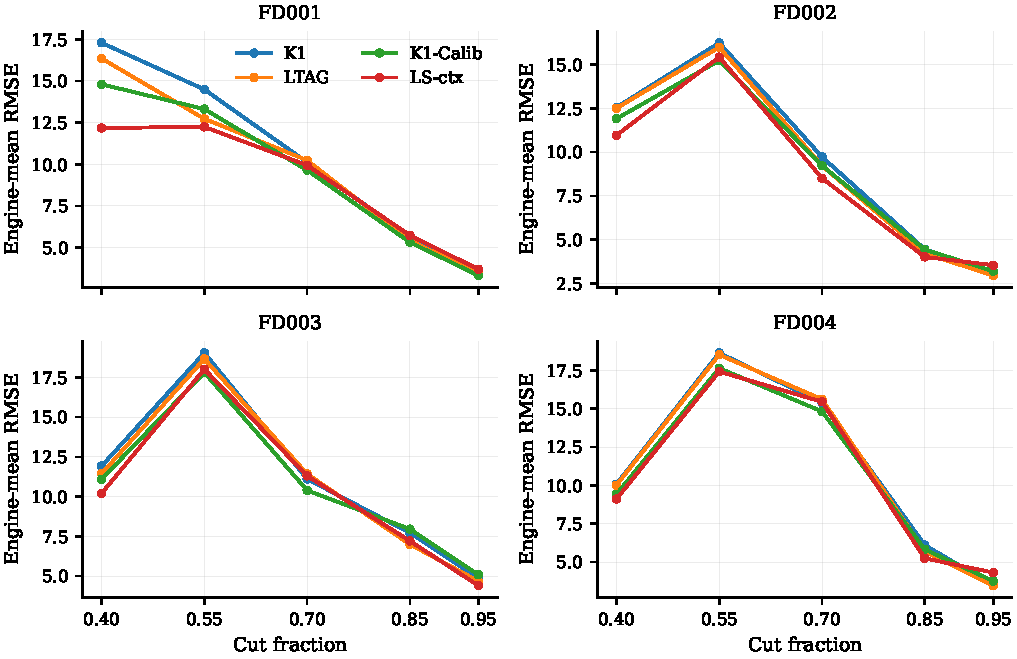
\includegraphics[width=0.95\textwidth]{figures/fig1_cutwise.pdf}
    \caption{Cut-wise engine-mean RMSE on the validation engines for K1, LTAG,
    K1-Calib, and LS-ctx. The calibration methods (K1-Calib, LS-ctx) are stronger
    at early cuts (0.40--0.55); near end-of-life (0.85--0.95) LTAG is competitive
    with or better than the calibration baselines. This crossover explains why a
    single mean over all cuts can rank the methods differently from the
    end-of-life test.}
    \label{fig:cutwise}
\end{figure*}

% === Fig 2: frozen B0 test RMSE ===
\begin{figure}[t]
    \centering
    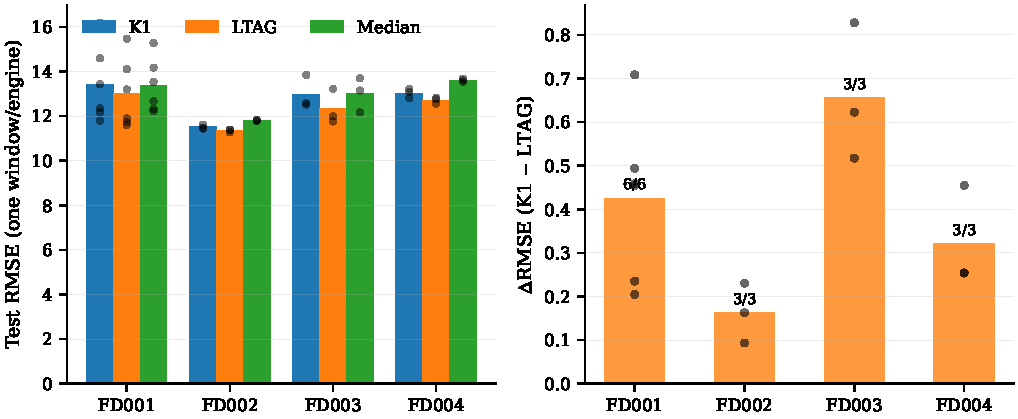
\includegraphics[width=0.48\textwidth]{figures/fig2_test.pdf}
    \caption{Frozen B0 test RMSE (one window per engine). Bars are subset means;
    dots are individual seeds (FD001: 6 seeds; FD002--FD004: 3 seeds). LTAG is
    lower than K1 on all four subsets (15/15 seed-subset wins; mean improvement
    +0.391).}
    \label{fig:test}
\end{figure}

% === Fig 3: per-engine delta RMSE ===
\begin{figure}[t]
    \centering
    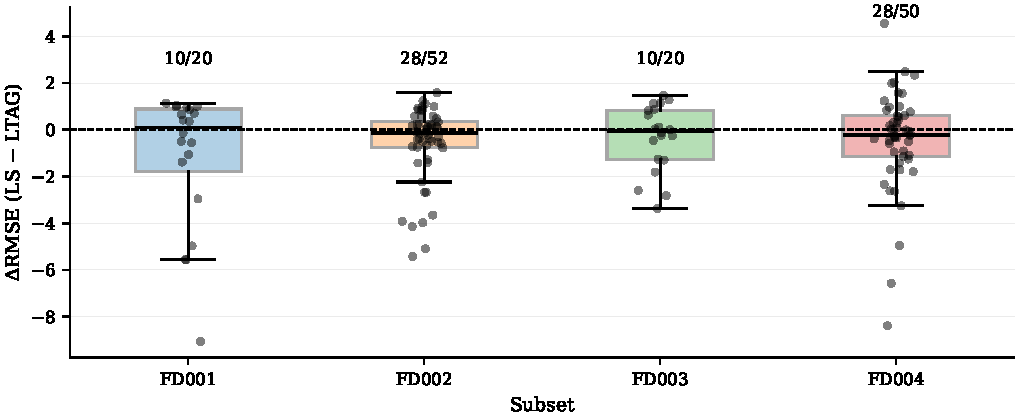
\includegraphics[width=0.48\textwidth]{figures/fig3_winrate.pdf}
    \caption{Per-engine $\Delta$RMSE (LS-ctx $-$ LTAG) on validation. Positive values
    mean LTAG is better. LS-ctx wins on only 10/20, 28/52, 10/20, and 28/50 engines;
    the mean gain is driven by a minority of high-error engines, and the FD001
    median is slightly worse for LS-ctx.}
    \label{fig:winrate}
\end{figure}
